\documentclass{beamer}
\usetheme{Malmoe}
\usecolortheme{dove}
%\setbeamertemplate{navigation symbols}{}  %remove navigation symbols
%Deutsch
\usepackage[ngerman]{babel}
\usepackage[utf8]{inputenc}
%Mathe
\usepackage{amsmath}
%Einheiten
\usepackage{siunitx}
%Baumstrukturen
\usepackage{tikz}
\usepackage{tikz-qtree}
\usepackage{textcomp}   % allows \textrightarrow
%Bildquellen
\usepackage{varwidth}
\usepackage{graphicx}
\usepackage{hyperref}

\author{Florian Seligmann}
\title{Die Baupolitik des Augustus}
\date{\textbf{11.6.2018}}

\tikzset{
  invisible/.style={opacity=0},
  visible on/.style={alt={#1{}{invisible}}},
  alt/.code args={<#1>#2#3}{%
    \alt<#1>{\pgfkeysalso{#2}}{\pgfkeysalso{#3}}
  }
}

%Item mit Pfeil
\newcommand{\aitem}{%
\item[$\rightarrow$]
}

%Bildquellen
\newcommand*{\quelle}{%
  \tiny Quelle:
}

%Bilder
\newcommand{\bild}[3]{%
	\begin{figure}
	\centering
  \begin{varwidth}{\linewidth}
    \raggedleft
    \includegraphics[scale=#2, width=\textwidth]{#1}\\
    \quelle{\url{#3}}
  \end{varwidth}
\end{figure}
}
\newcommand{\fbild}[3]{%
	\begin{figure}
	\centering
  \begin{varwidth}{\linewidth}
    \raggedleft
    \includegraphics[scale=#2]{#1}\\
    \quelle{\url{#3}}
  \end{varwidth}
\end{figure}
}

%Einheiten
\sisetup{
  locale = DE ,
  per-mode = symbol
}

%=====================================================================================================================================
\begin{document}

\frame{\titlepage}
\frame{\frametitle{Gliederung}
\tableofcontents
} %End of frame
%-------------------------------------------------------------------------------------------------------------------------------------

%----------------------------------------------Res gestae---------------------------

\frame{\frametitle{Primärquelle - Re gestae}  % http://www.latein-imperium.de/include.php?path=content&mode=print&contentid=126
	\begin{itemize}
		\item Wichtigste Primärquelle: \glqq{}Res gestae Divi Augusti\grqq{}  % Taten des göttliche Augustus
		\item Verfasst mit 76 von Augustus
		\item Aufgestellt im ganzen Reich
		\item Ziel: Macht nicht selbst erstrebt, immer vom Senat \& Volk freiwillig übertragen
	\end{itemize}
}%eof

%----------------------------------------------------------------------------------

\section{Entwicklung der Baupolitik}

\subsection{Zeit der Bürgerkriege}

\frame{\frametitle{Bürgerkriege}
	\begin{itemize}
		\item 44 v. Chr. - 31 v. Chr.
		\pause
		\item Antonius von Ägypten aus
		\aitem Betonung Roms
		\pause
		\aitem Repräsentative Bauten in Rom
		\aitem Caesarkult
	\end{itemize}
}%eof

\frame{\frametitle{Beispiele zur Zeit der Bürgerkriege}
	%Mausoleum Augustus auf Marsfeld
	\begin{center}
		\bild{images/mausoleum_beschnitten.png}{0.5}{http://www.roma-antiqua.de/abbildungen/antikes_rom/marsfeld/2000_351.jpg}
		%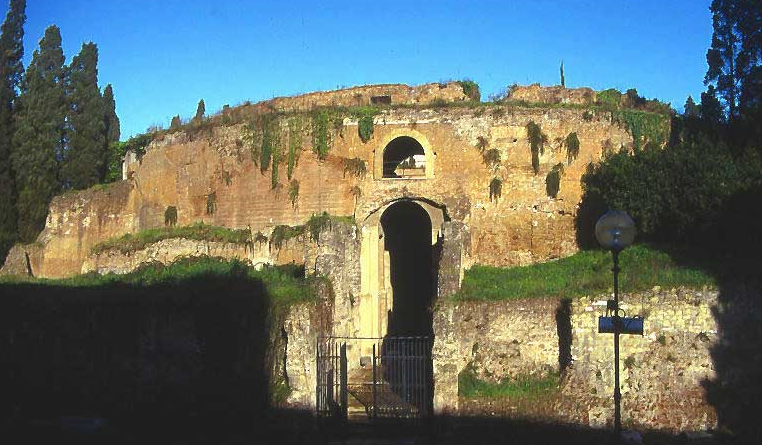
\includegraphics[0.5]{images/mausoleum_beschnitten.png}
	\end{center}
	
}%eof

\frame{\frametitle{Beispiele zur Zeit der Bürgerkriege}
	%Mausoleum Augustus auf Marsfeld
	\bild{images/mausoleum_oben.png}{1.0}{https://www.realmofhistory.com/wp-content/uploads/2017/05/restoration-mausoleum-of-augustus-rome_3-770x437.jpg}
}%eof

\frame{\frametitle{Bürgerkriege}
	\begin{itemize}
		\item Bezug zu Apollo
		\pause
		\item Betonung der Ahnenreihe
		\pause
		\item Über Venus, Aeneas, Iulus Ascanius und Caesar
		\aitem Curia Iulia, Tempel des Divus Iulius auf dem Forum Romanum %Curia Iulia: Senatsgebäude, von Caesar begonnen; Divus Iulius: Tempel für vergöttlichten Caesar -> Lage am Forum Romanum
		\pause
		\item Bezug zu Romulus $\rightarrow$ \glqq{}Neubegründer\grqq{}
		\aitem Wohnhaus auf dem Palatin bei der Hütte des Romulus
	\end{itemize}
}%eof

\subsection{Zeit des Prinzipats}

\frame{\frametitle{Prinzipat}
	\begin{quote}
		Da die Stadt nicht so prunkvoll aussah, wie es die Bedeutung des Imperiums verlangte, auch immer wieder von Überflutungen und 				Feuersbrünsten bedroht wurde, verschönerte er sie so, dass er danach mit Recht behaupten konnte, er habe ein Rom aus Ziegeln vorgefunden und eines aus Marmor hinterlassen. (...)
	\end{quote}
	\tiny{Suet. Aug. 28, 3}	%Kaiserbiographien
}%eof

\frame{\frametitle{Prinzipat}
	\begin{itemize}
		\pause
		\item Erneuerung der Infrastruktur %-> Agrippa; "Cloaca Maxima"; Aquaedukte; Straßen; Brandschutz
		\pause
		\item Erneuerung der Tempel %-> Rückkehr zu den Göttern, vor allem Iupiter, Mars, Apollo
		\pause
		\item Fertigstellung vieler Bauwerke
		\pause
		\item Siegesdenkmäler
	\end{itemize}
}%eof

\frame{\frametitle{Marmor}
	\begin{itemize}
		\item Marmor während Republik kaum verwendet
		\item Marmor Symbol für \glqq{}Goldenes Zeitalter\grqq{}.
		\item Kontrolle der Seewege $\rightarrow$ Marmor aus dem ganzen Reich % Machtrepräsentation
		\item Marmor sehr teuer $\rightarrow$ Gebäude oft nur mit Marmor verkleidet
	\end{itemize}
}%eof

\frame{\frametitle{Übersetzung - Teil 1}
	\begin{columns}
		\begin{column}{0.5\textwidth}
			Bella terrā et mari civilia externaque toto in orbe terrarum saepe gessi, victorque omnibus veniam petentibus civibus peperci. Externas gentes, quibus tuto ignosci potuit, conservare quam excidere malui. (…)
		\end{column}
		\begin{column}{0.5\textwidth}
			Oft habe ich auf dem ganzen Erdkreis zu Land und zur See bürgerliche und auswärtige Kriege geführt, und als Sieger verschonte ich
alle um Schonung bittenden Bürger. Ich habe es vorgezogen, ausländische Stämme, denen gefahrlos verziehen werden konnte, zu bewahren 
anstatt sie zu vernichten.
		\end{column}
	\end{columns}
}%eof

%Ianus Quirinus -> Quirinus: Altrömischer Kriegsgott
\frame{\frametitle{Übersetzung - Teil 2}
	\begin{columns}
		\begin{column}{0.5\textwidth}
			Ianum Quirinum, quem clausum esse maiores nostri voluerunt cum per totum imperium populi Romani terra marique esset parta victoriis pax, cum priusquam nascerer, a condita urbe bis omnino clausum fuisse prodatur memoriae, ter me principe senatus claudendum esse censuit. (…)
		\end{column}
		\begin{column}{0.5\textwidth}
			Der (Tempel des) Ianus Quirinus, von dem unsere Vorfahren wollten, dass er geschlossen sei, wenn im ganzen Reich des römischen
Volkes zu Land und zur See durch Siege erworbener Friede sei,
der, bevor ich geboren wurde, von der Gründung der Stadt an überhaupt nur zweimal geschlossen
gewesen sein soll, beschloss der Senat unter meinem Prinzipat dreimal zu schließen.
		\end{column}
	\end{columns}
}%eof

%highlited
\frame{\frametitle{Übersetzung - Teil 2}
	\begin{columns}
		\begin{column}{0.5\textwidth}
			\textbf{Ianum Quirinum}, quem clausum esse maiores nostri voluerunt cum per totum imperium populi Romani terra marique esset parta victoriis pax, cum priusquam nascerer, a condita urbe bis omnino clausum fuisse prodatur memoriae, ter me principe senatus claudendum esse censuit. (…)
		\end{column}
		\begin{column}{0.5\textwidth}
			\textbf{Der (Tempel des) Ianus Quirinus}, von dem unsere Vorfahren wollten, dass er geschlossen sei, wenn im ganzen Reich des römischen Volkes zu Land und zur See durch Siege erworbener Friede sei, der, bevor ich geboren wurde, von der Gründung der Stadt an überhaupt nur zweimal geschlossen gewesen sein soll, beschloss der Senat unter meinem Prinzipat dreimal zu schließen.
		\end{column}
	\end{columns}
}%eof


\frame{\frametitle{Janustempel}
	\begin{itemize}
		\item Ursprünglich ein Holzbau, unter Augustus aus Bronze neu errichtet
		\pause
		\item Ursprünglich aus mythischer Vorzeit
		\item Kein echter Tempel %Durchgangsbogen -> ianus; nicht aedes
		\pause
		\item Ianus: Gott des Anfangs und Endes %Davor: Stück Land, das symbolisch zu Feindesland deklariert werden konnte -> Speerwurf
		\pause
		\item Tore bei Frieden im ganzen Reich geschlossen %durch Siege errungener Friede
		\pause
		\aitem Eventuell von Augustus selbst eingeführter Brauch
	\end{itemize}
}%eof
%===================================================================================================

\section{Ara Pacis Augustae}

\frame{\frametitle{Übersetzung - Teil 3}
	\begin{columns}
		\begin{column}{0.5\textwidth}
			Cum ex Hispania Galliaque, rebus in iis provincis prospere gestis, Romam redii, Ti. Nerone P. Qintilio consulibus, aram Pacis Augustae senatus pro reditu meo consacrandam censuit ad campum Martium, in qua magistratus et sacerdotes virginesque Vestales anniversarium sacrificium facere iussit.
		\end{column}
		\begin{column}{0.5\textwidth}
			Als ich aus Spanien und Gallien, nachdem ich in diesen (Provinzen) Taten glücklich vollbracht hatte, nach Rom 13 v. Chr. (im 
Konsulatsjahr des Tiberius Nero und Publius Quintilius) zurückkehrte, stimmte der Senat zu Ehren meiner Rückkehr für die Weihung eines Altars des Friedens des Augustus auf dem Marsfeld, in dem Beamte, Priester und Vestalinnen jährlich auf Befehl ein Opfer darbringen sollten.
		\end{column}
	\end{columns}
}%eof

%highlited
\frame{\frametitle{Übersetzung - Teil 3}
	\begin{columns}
		\begin{column}{0.5\textwidth}
			Cum ex Hispania Galliaque, rebus in iis provincis prospere gestis, Romam redii, Ti. Nerone P. Qintilio consulibus, \textbf{aram Pacis Augustae} senatus pro reditu meo consacrandam censuit ad campum Martium, in qua magistratus et sacerdotes virginesque Vestales anniversarium sacrificium facere iussit.
		\end{column}
		\begin{column}{0.5\textwidth}
			Als ich aus Spanien und Gallien, nachdem ich in diesen (Provinzen) Taten glücklich vollbracht hatte, nach Rom 13 v. Chr. (im 
Konsulatsjahr des Tiberius Nero und Publius Quintilius) zurückkehrte, stimmte der Senat zu Ehren meiner Rückkehr für die Weihung eines \textbf{Altars des Friedens des Augustus} auf dem Marsfeld, in dem Beamte, Priester und Vestalinnen jährlich auf Befehl ein Opfer darbringen sollten.
		\end{column}
	\end{columns}
}%eof

\frame{\frametitle{Ara Pacis Augustae}
	\bild{images/ap_totale.png}{0.35}{https://www.bluffton.edu/homepages/facstaff/sullivanm/italy/rome/arapacis/0081.jpg}
}%eof


\frame{\frametitle{Ara Pacis Augustae - Eckdaten}
	\begin{itemize}
		\item 13 v. Chr. vom Senat in Auftrag gegeben
		\item Standort: Marsfeld, neben Pantheon, Marcellustheater und Augustusmausoleum
		\item Geweiht am 30. Januar 9 v. Chr. (Geburtstag der Livia)
		\pause
		\item 11.63m x 10.62m
		\pause
		\item Aufbau ähnlich einem \glqq{}templum minus\grqq{} %früher Holzzaun um Altar in der Mitte
		\aitem Aber aus massivem lunensischem Marmor % Carrara-Marmor, wg. Provin Luna
	\end{itemize}
} %eof

\frame{\frametitle{Fundgeschichte}
	\begin{itemize}
		\item Unter Tiberschlamm begraben
		\pause
		\item 1568 Erste Entdeckungen
		\item 1879 Indentifikation als Ara Pacis
		\pause
		\item Ausgrabungen 1903 \& 1937/38 %Mussolini -> Identifikation mit Augustus
		\item Heute Rekonstruktion
	\end{itemize}
}%eof

\frame{\frametitle{Aufgaben}
	\begin{itemize}
		\item Rückblick auf Griechenland \& die Republik
		\item Versprechen eines \glqq{}Goldenen Zeitalters\grqq{} 
	\end{itemize}
}%eof

\frame{\frametitle{Gestaltung}
	\begin{itemize}
		\item Reliefs auf Außen- und Innenseite
		\item Wahrscheinlich griechische Künstler %wg. Detailgenauigkeit -> Sittenverfall durch griechische Kunst 
		\item Interpretation sehr umstritten
		\item Einteilung %Oben Szenen, Handlungen; unten Natur, Wildheit, Roheit /Blütezeit
	\end{itemize}
}%eof

\frame{\frametitle{Gestaltung}
	%\bild{images/arapacis_plan.png}{1.0}{http://www.lingualatina.de/bilder/arapacis.jpg}
	\begin{figure}
		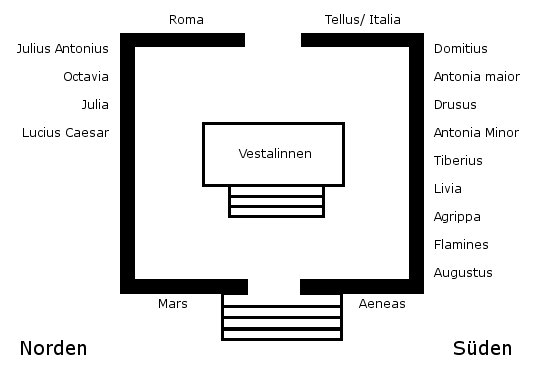
\includegraphics[height=0.8\textheight]{images/arapacis_plan.png}\\
		\quelle{\url{http://www.lingualatina.de/bilder/arapacis.jpg}}
	\end{figure}
}%eof

%--------------------------------------------horologium-----------------
\frame{\frametitle{Horologium solarium Augusti}
	\begin{figure}
		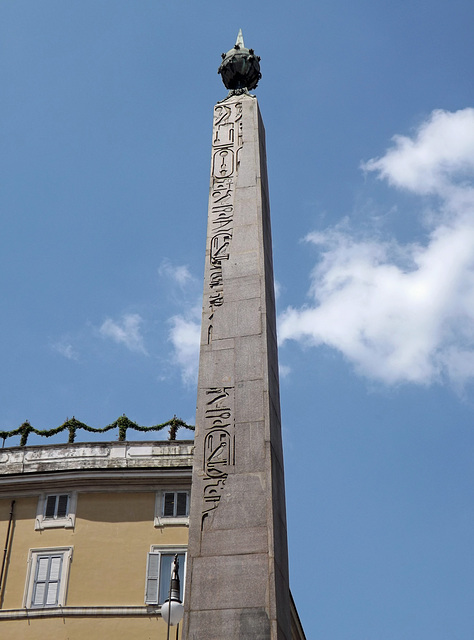
\includegraphics[height=0.8\textheight]{images/horologium.png}\\
		\quelle{\url{http://cdn.ipernity.com/134/84/75/24228475.ef26a17d.640.jpg?r2}}
	\end{figure}
}%eof
\frame{\frametitle{Horologium solarium Augusti}
	\begin{itemize}
		\item Größte Sonnenuhr Roms
		\item Beute aus Ägypten $\rightarrow$ Sieg über Kleopatra
		\pause
		\item Schatten am 23. September in Eingang der Ara pacis % Augustus GB -> 'Zeichen der Götter' -> Apollo (Gott der Sonne)
		\item 
	\end{itemize}
}%eof

%-----------------------Auswirkungen-----------------------------
\section{Auswirkungen der Baupolitik}

\frame{\frametitle{Auswirkungen}
		\begin{itemize}
			\pause
			\item Wettbewerb unter wohlhabenden Bürgern
			\aitem Sichtbares \glqq{}Goldenes Zeitalter\grqq{}
		\end{itemize}
}%eof
\end{document}